\section{Empirical Demonstration}

The framework is demonstrated on a graph routing problem. The goal is not to evaluate routing algorithms, but to show how the decision-valued map makes representational dependence observable in a concrete setting.

\subsection{Setup}

The demonstration fixes a directed graph with node set $V$ where $|V| = 564$, edge set $E$, immutable edge attributes including baseline costs derived from geographic distance and a normalized stress metric. The snapshot is content-addressed and frozen before any engine execution. A single origin-destination query is fixed at start node 85 and end node 50.

Each representation encodes the graph's edge costs as a deterministic function of the frozen edge attributes. Two representation parameters control the cost surface. The first, neighbor weight, applies a weight to a neighbor-based cost component and is tested at 0.5 and 1.0. The second, second-order weight, applies a weight to a second-order cost component and is tested at 0.25 and 0.5. Each sweep varies one parameter while holding the other fixed, producing two representation variants per sweep and four engine evaluations total.

The engine is a fixed shortest-path solver using Dijkstra's algorithm~\cite{dijkstra1959note}, with configuration and version held constant across all runs. Execution times ranged from 0.5 to 1.4 milliseconds. The equivalence policy, version 1.0.0, performs exact match on the canonicalized node sequence of the computed route. Two routes are assigned the same decision identity if and only if they traverse identical node sequences. The policy uses SHA-256 over JSON-serialized, sorted-key, UTF-8-encoded route nodes.

\subsection{Results}

The neighbor weight sweep varies the neighbor weight from 0.5 to 1.0 while holding second-order weight fixed at 0.25. Both representations yield the same route, Decision~A, a 16-node path:
\[
[85,\; 176,\; 463,\; 14,\; 404,\; 76,\; 406,\; 407,\; 223,\; 200,\; 311,\; 310,\; 314,\; 322,\; 323,\; 50].
\]
Doubling the neighbor weight from 0.5 to 1.0 does not change route identity. This parameter range constitutes a persistence region under the tested policy.

The second-order weight sweep varies the second-order weight from 0.25 to 0.5 while holding neighbor weight fixed at 0.5. At second-order weight 0.25, the engine produces Decision~A. At second-order weight 0.5, the engine produces Decision~B, a 14-node path:
\[
[85,\; 411,\; 419,\; 422,\; 332,\; 204,\; 500,\; 369,\; 79,\; 402,\; 473,\; 502,\; 501,\; 50].
\]
The route changes entirely, traversing a different region of the graph. The boundary between these two decision identities lies between second-order weight values 0.25 and 0.5. This is a fracture, where a small parameter change induces a qualitative change in the discrete outcome. Table~\ref{tab:sweep-summary} summarizes the sweep results; Figure~\ref{fig:persistence-fracture} shows the persistence and fracture structure.

\begin{table}[t]
\centering
\caption{Representational sweep results.}
\label{tab:sweep-summary}
\smallskip
\tablestyle
\rowcolors{2}{tableShade}{white}
\begin{tabular}{@{\hskip 8pt}l l c c l@{\hskip 8pt}}
\toprule
\rowcolor{white}
Sweep parameter & Value & Decision & Nodes & Boundary \\
\midrule
neighbor weight & 0.5 & A & 16 & \\
neighbor weight & 1.0 & A & 16 & No \\
second-order weight & 0.25 & A & 16 & \\
second-order weight & 0.5 & B & 14 & Yes \\
\bottomrule
\end{tabular}
\end{table}

\begin{figure}[t]
  \centering
  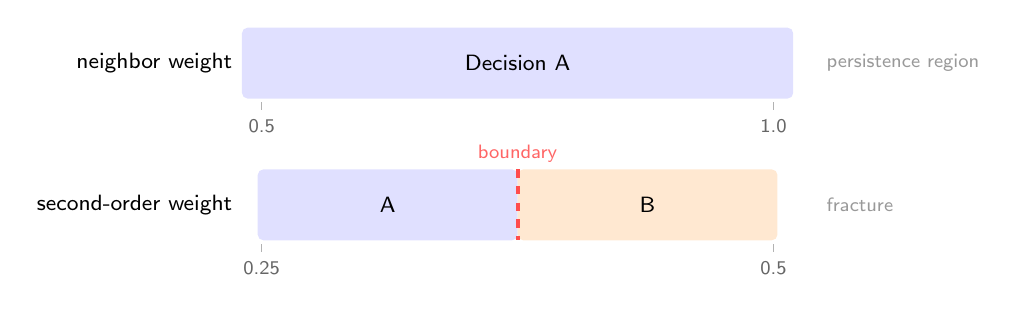
\begin{tikzpicture}[
    region/.style={minimum height=9mm, align=center, font=\sffamily\footnotesize, rounded corners=2pt},
    regionA/.style={region, fill=blue!12},
    regionB/.style={region, fill=orange!18},
    lbl/.style={font=\sffamily\footnotesize, anchor=east},
    tick/.style={font=\sffamily\scriptsize, text=black!60},
    plbl/.style={font=\sffamily\scriptsize, text=black!40, anchor=west}
  ]

  % Panel (a): Neighbor weight - persistence
  \node[lbl] at (-0.3, 0) {neighbor weight};
  \node[regionA, minimum width=70mm] at (3.2, 0) {Decision A};
  \node[tick, anchor=north] at (-0.05, -0.6) {0.5};
  \node[tick, anchor=north] at (6.45, -0.6) {1.0};
  \draw[black!30] (-0.05, -0.5) -- (-0.05, -0.6);
  \draw[black!30] (6.45, -0.5) -- (6.45, -0.6);
  \node[plbl] at (7.0, 0) {persistence region};

  % Panel (b): Second-order weight - fracture
  \node[lbl] at (-0.3, -1.8) {second-order weight};
  \node[regionA, minimum width=33mm] at (1.55, -1.8) {A};
  \node[regionB, minimum width=33mm] at (4.85, -1.8) {B};
  \node[tick, anchor=north] at (-0.05, -2.4) {0.25};
  \node[tick, anchor=north] at (6.45, -2.4) {0.5};
  \draw[black!30] (-0.05, -2.3) -- (-0.05, -2.4);
  \draw[black!30] (6.45, -2.3) -- (6.45, -2.4);
  \node[plbl] at (7.0, -1.8) {fracture};

  % Fracture marker
  \draw[red!70, line width=1.5pt, dashed] (3.2, -1.35) -- (3.2, -2.25);
  \node[font=\sffamily\scriptsize, text=red!60, fill=white, inner sep=1pt, anchor=south] at (3.2, -1.3) {boundary};

  \end{tikzpicture}
  \caption{Identity persistence and fracture structure for the two representation parameters. The neighbor weight parameter spans a single persistence region in which both tested values produce Decision~A, indicating route identity is stable across this range. The second-order weight parameter spans two regions separated by a fracture, where route identity changes from Decision~A to Decision~B between the values 0.25 and 0.5. The exact threshold is not resolved by this two-point sample.}
  \label{fig:persistence-fracture}
\end{figure}

\subsection{Replay Verification}

Replay verification is performed on a decision produced by the sweep. The procedure reloads the stored raw output and policy specification, recomputes all three identifying fields so as to check them against the persisted values. All recomputed values match exactly, as shown in Table~\ref{tab:replay} and Figure~\ref{fig:replay}.

\begin{table}[t]
\centering
\caption{Replay verification results.}
\label{tab:replay}
\smallskip
\tablestyle
\rowcolors{2}{tableShade}{white}
\begin{tabular}{@{\hskip 8pt}l l l@{\hskip 8pt}}
\toprule
\rowcolor{white}
Field & Persisted & Recomputed \\
\midrule
Policy ID & pol\_d8da3e00e9584eb1 & pol\_d8da3e00e9584eb1 \\
Payload hash & 3a9d63ac28378116 & 3a9d63ac28378116 \\
Decision ID & dec\_e28092c4dc33b8f1 & dec\_e28092c4dc33b8f1 \\
\bottomrule
\end{tabular}
\end{table}

The replay writes no new rows and modifies no database state. Table counts before and after replay are identical, with 1~engine run, 1~decision, 1~f\_map entry. This confirms that the content-addressing chain from raw output through policy application to decision identity is deterministic and end-to-end auditable.

\begin{figure}[t]
  \centering
  \begin{tikzpicture}[
    node distance=8mm,
    rbox/.style={draw, rounded corners, align=center, inner sep=6pt, text width=34mm, font=\sffamily\small, fill=blue!6},
    arrow/.style={-Latex, thick},
    ann/.style={font=\sffamily\scriptsize, text=black!50, align=center}
  ]

  \node[rbox] (s1) {Persisted\\decision record};
  \node[rbox, right=10mm of s1] (s2) {Reload and\\recompute};
  \node[rbox, right=10mm of s2, fill=tableShade] (s3) {Equality check};

  \draw[arrow] (s1) -- (s2);
  \draw[arrow] (s2) -- (s3);

  \node[ann, below=4mm of s1] {stored artifact URI,\\policy specification};
  \node[ann, below=4mm of s2] {recompute policy ID,\\payload hash, decision ID};
  \node[ann, below=4mm of s3] {read-only, 0 writes\\PASS / FAIL};

  \end{tikzpicture}
  \caption{Replay verification pipeline. A persisted decision record is used to reload the raw output artifact and policy specification. All three identifying fields are recomputed from stored artifacts and compared against persisted values. The procedure is read-only and writes no database rows; a successful pass confirms deterministic self-consistency of the content-addressing chain.}
  \label{fig:replay}
\end{figure}
